% \documentclass[10pt,notes,mathserif]{beamer}
% \setbeameroption{show notes on second screen}
% \setbeamertemplate{note page}{\insertnote}

\documentclass[10pt,mathserif]{beamer}
\usepackage[utf8]{inputenc}

% Presentation specific stuff
\usetheme[progressbar=frametitle]{metropolis}

\usepackage[block=space,bibencoding=utf8,style=chem-rsc,maxbibnames=1,backend=biber]{biblatex}
% \usepackage[backend=biber,style=phys,maxcitenames=1,maxbibnames=2,giveninits=true]{biblatex}



\usepackage[font=footnotesize,labelformat=empty]{caption}
\usepackage{layouts}

% Math/physics notation stuff
\usepackage{svg}
\usepackage{amsmath}
\usepackage{amsfonts}
\usepackage{physics}
\usepackage{siunitx}
\usepackage{hyperref}
\usepackage{cleveref}
\usepackage{float}
\usepackage{subcaption}
\usepackage{stackengine}
\usepackage{calc}
\usepackage{xcolor}

% Misc
\usepackage[textsize=tiny,disable]{todonotes}
\usepackage{lipsum}

% Set up the biobliographies
\addbibresource{MPhys.bib}
\addbibresource{StochasticTopology.bib}
\renewcommand*{\bibfont}{\tiny}
\setbeamerfont{bibliography item}{size=\tiny}
\setbeamerfont{bibliography entry author}{size=\tiny}
\setbeamerfont{bibliography entry title}{size=\tiny}
\setbeamerfont{bibliography entry location}{size=\tiny}
\setbeamerfont{bibliography entry note}{size=\tiny}

\setlength\bibitemsep{0\itemsep}

\newcommand{\extra}[1]{\color{gray} #1 \normalcolor}
\newcommand{\mul}[1]{\underline{\smash{#1}}}
\newcommand{\subheading}[1]{\large\textbf{#1}\normalsize}

\begin{document}

\setlength{\abovedisplayskip}{1em}
\setlength{\belowdisplayskip}{0ex}

\begin{frame}
	\begin{flushright}
		
\includegraphics[width=0.4\textwidth]{figures/UCL_logo.pdf} \\
	\end{flushright}

	\vspace{2em}
	\LARGE
	Functional Dynamics in Out-of-Equilibrium Allosteric Assemblies \\
	\normalsize
	\vspace{1.5em}
	\small
	\emph{Jan Kocka, Jaime Agudo-Canalejo$^\dagger$, Kabir Husain$^\dagger$} \\
	% \vspace{.5em}
	\scriptsize
	Department of Physics and Astronomy, University College London \\
	\vspace{7em}

	\normalsize
	poster number: 2 \hfill
	\tiny $^\dagger$ indicates equal contribution

	\vfill
\end{frame}

\begin{frame}[fragile]{Allostery -- interactions between distant sites on a complex}
	\newrefsection
	\begin{figure}
		\centering
		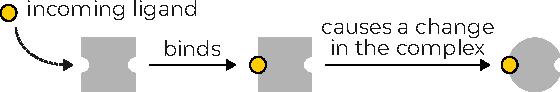
\includegraphics{figures/allostery_diagram.pdf}
	\end{figure}

	% \vspace{1em}

	\textbf{Notable examples:}
	\vspace{-.7em}
	\begin{itemize}
		\setlength\itemsep{0em}
		\item Cooperative binding in Haemoglobin \cite{stefanCooperativeBinding2013}
		\item Allosteric regulation in the Ribosome \cite{makarovaRibosomeAllostericallyRegulated2017}
		      % \item `Second secret of life`\cite{fentonAllosteryIllustratedDefinition2008}
	\end{itemize}

	\textbf{Multiple established equilibrium models:}
	\vspace{-.7em}
	\begin{itemize}
		\setlength\itemsep{0em}
		\item Monod-Wyman-Changeux (MWC)\cite{monodNatureAllostericTransitions1965}
		\item Koshland-Nemethy-Filmer (KNF)\cite{koshlandComparisonExperimentalBinding1966}
	\end{itemize}

	\vfill
	\printbibliography[heading=none]
	\vspace{-\fill}
\end{frame}

\begin{frame}[fragile]{What does out-of-equilibrium allostery allow}
	\newrefsection

	\vspace{1em}

	\textbf{But there are out-of-equilibrium allosteric systems:}
	\vspace{-.7em}
	\begin{itemize}
		\setlength\itemsep{0em}
		\item KaiC circadian clock\cite{vanzonAllostericModelCircadian2007}
		\item DNA Clamp Loader\cite{kelchHowDNAPolymerase2011}
	\end{itemize}

	\vspace{1.5em}

	\begin{center}
		\bf
		\large
		% What kinds of new behaviour does a non-equilibrium drive allow?
		What classes of new behaviour are possible in out-of-equilibrium allostery?
		% What classes of new behaviour does out-of-equilibrium drive allow in allosteric systems?
	\end{center}

	\vspace{1em}

	\vfill
	\printbibliography[heading=none]
	\vspace{-\fill}
\end{frame}

\begin{frame}[fragile]{We construct minimal models capable of allostery}
	\newrefsection

    \vspace{3em}
	\textbf{Core ingredients in our approach}
	\vspace{-0.5em}
	\begin{itemize}
		\item Systems made of identical subunits %, capable of conformation changes and binding ligands
		\item Local interactions \extra{(nearest-neighbor)}
		\item Thermodynamically consistent \extra{(local detailed balance)}
		      % \item Master equation statistical physics models with graph theory analysis
	\end{itemize}
    \vspace{2em}
    \begin{center}
		
\includegraphics[width=0.7\textwidth]{figures/our_approach_diagram.pdf}
    \end{center}
\end{frame}

\begin{frame}[fragile]{Topologically protected dynamic states?}
	\newrefsection
	\begin{figure}
		\centering
		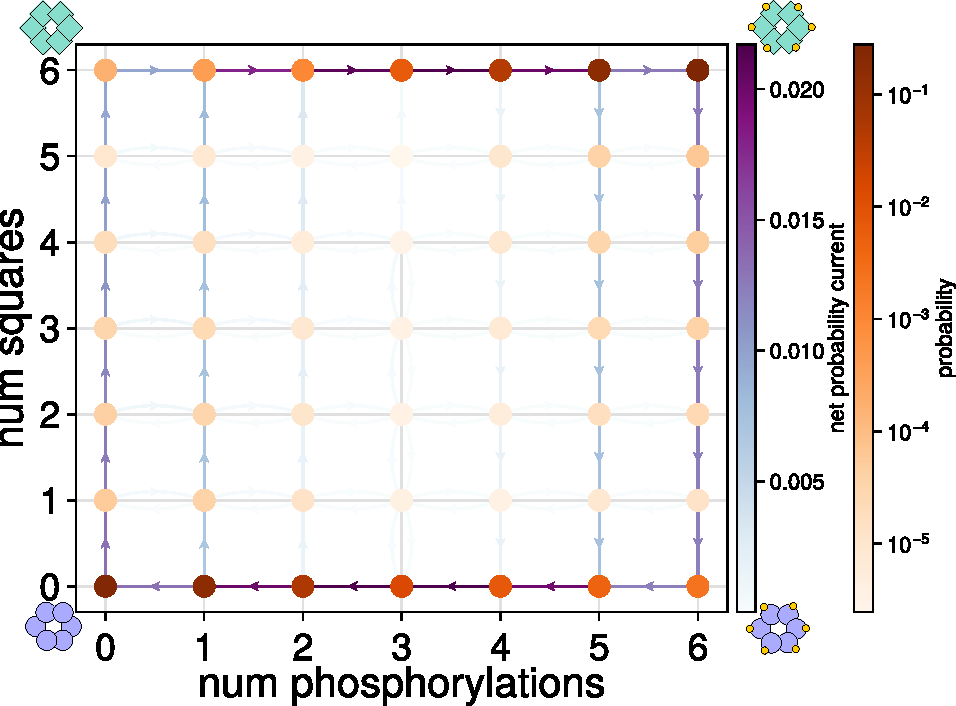
\includegraphics[width=0.9\textwidth]{figures/ca_plot_plus_diagrams.pdf}
		% 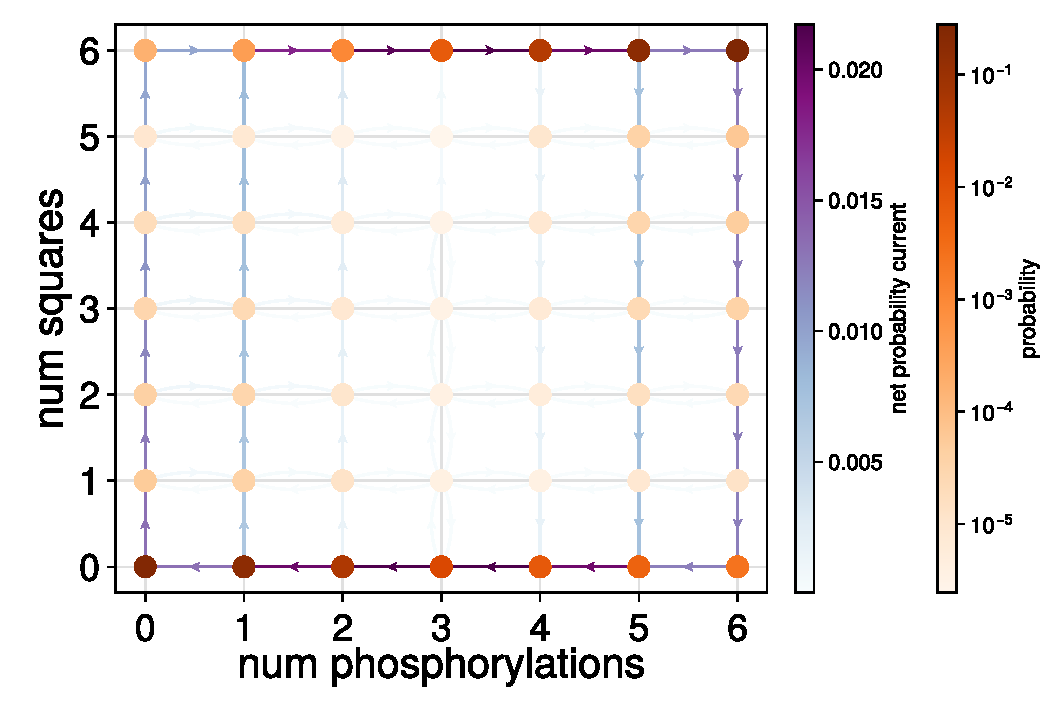
\includegraphics[width=0.8\textwidth]{figures/ca_square.pdf}
		\caption{
			Each node is a measurable group of states, their colours denoting steady state probability, and the arrows are the steady state probability currents.
		}
	\end{figure}
	\vfill
	\printbibliography[heading=none]
	\vspace{-\fill}
\end{frame}

\begin{frame}[fragile]{Chirality induced by out-of-equilibrium drive}
	\newrefsection
	\begin{figure}
		\centering
        \begin{subfigure}{0.49\textwidth}
			\centering
			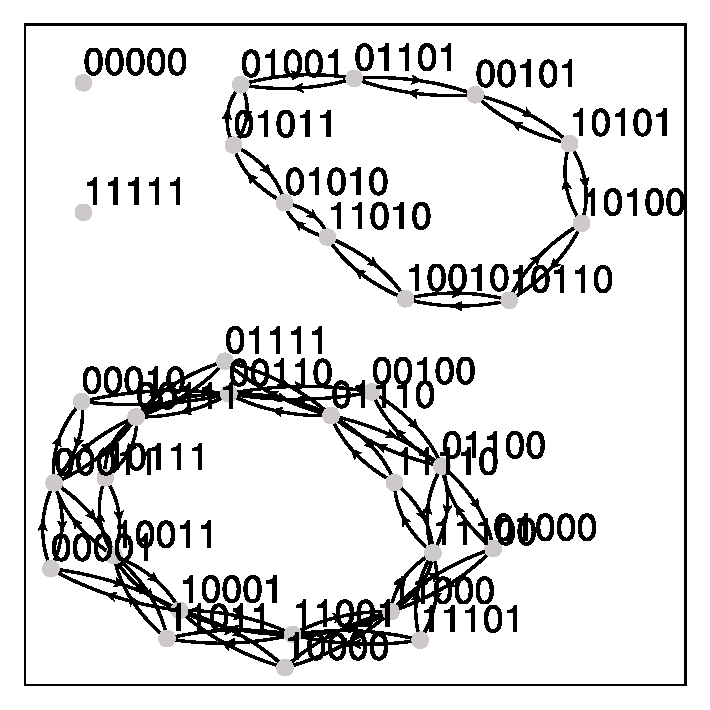
\includegraphics[width=\textwidth]{figures/ned_r150_N5_square.pdf}
            \caption{
                Equilibrium ruleset, diffusion on loops
            }
		\end{subfigure}
        \begin{subfigure}{0.49\textwidth}
			\centering
			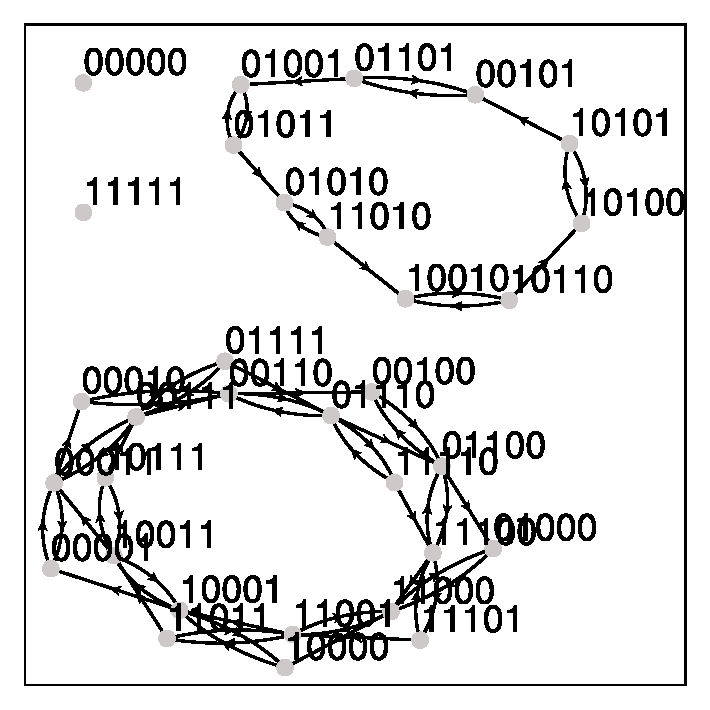
\includegraphics[width=\textwidth]{figures/ned_r134_N5_square.pdf}
            \caption{
                Non-equilibrium ruleset, directed currents
            }
		\end{subfigure}
	\end{figure}
\end{frame}

\begin{frame}
	\begin{flushright}
		
\includegraphics[width=0.4\textwidth]{figures/UCL_logo.pdf} \\
	\end{flushright}

	\vspace{2em}
	\begin{center}
		\LARGE
		Thank you for your attention
	\end{center}
	\normalsize
	\vspace{10.5em}

	\normalsize
	poster number: 2

	\vfill
\end{frame}


\end{document}
